\documentclass[.../Dokumentation.tex]{subfiles}
\begin{document}
\subsection{Projektidee}\label{sec-intr-idea}
Es soll eine Kombination aus Eingabegerät und Darstellung geschaffen werden, 
die sich grob an der Bewegung von Spielzeug-Autos auf einem 
mit einer abstrakten Stadt und ihrer Verkehrsinfrastruktur bedruckten Teppich 
orientiert. Gleichzeitig soll maßstabsgetreu die Bewegung der Fahrzeuge 
aufgenommen und in ihre entsprechende CO\textsubscript{2}-Emmission übersetzt 
werden. Die so anfallende Belastung für die Umwelt soll auf einem Display 
optisch ansprechend aufbereitet und mit anschaulichen, zusätzlichen 
Informationen zusammengebracht werden. 
Hierdurch sollen die Konsequenzen des eigenen Handelns verdeutlicht 
und so einem Nutzer näher gebracht werden können, als es durch das 
Auflisten von Statistiken oder Ähnlichem möglich wäre. In Abbildung 
\ref{fig-sponge} ist ein erster \textit{Low-Fidelity}-Prototyp der hier 
beschriebenen Idee zu sehen
\begin{figure}[H]
    \begin{center}
    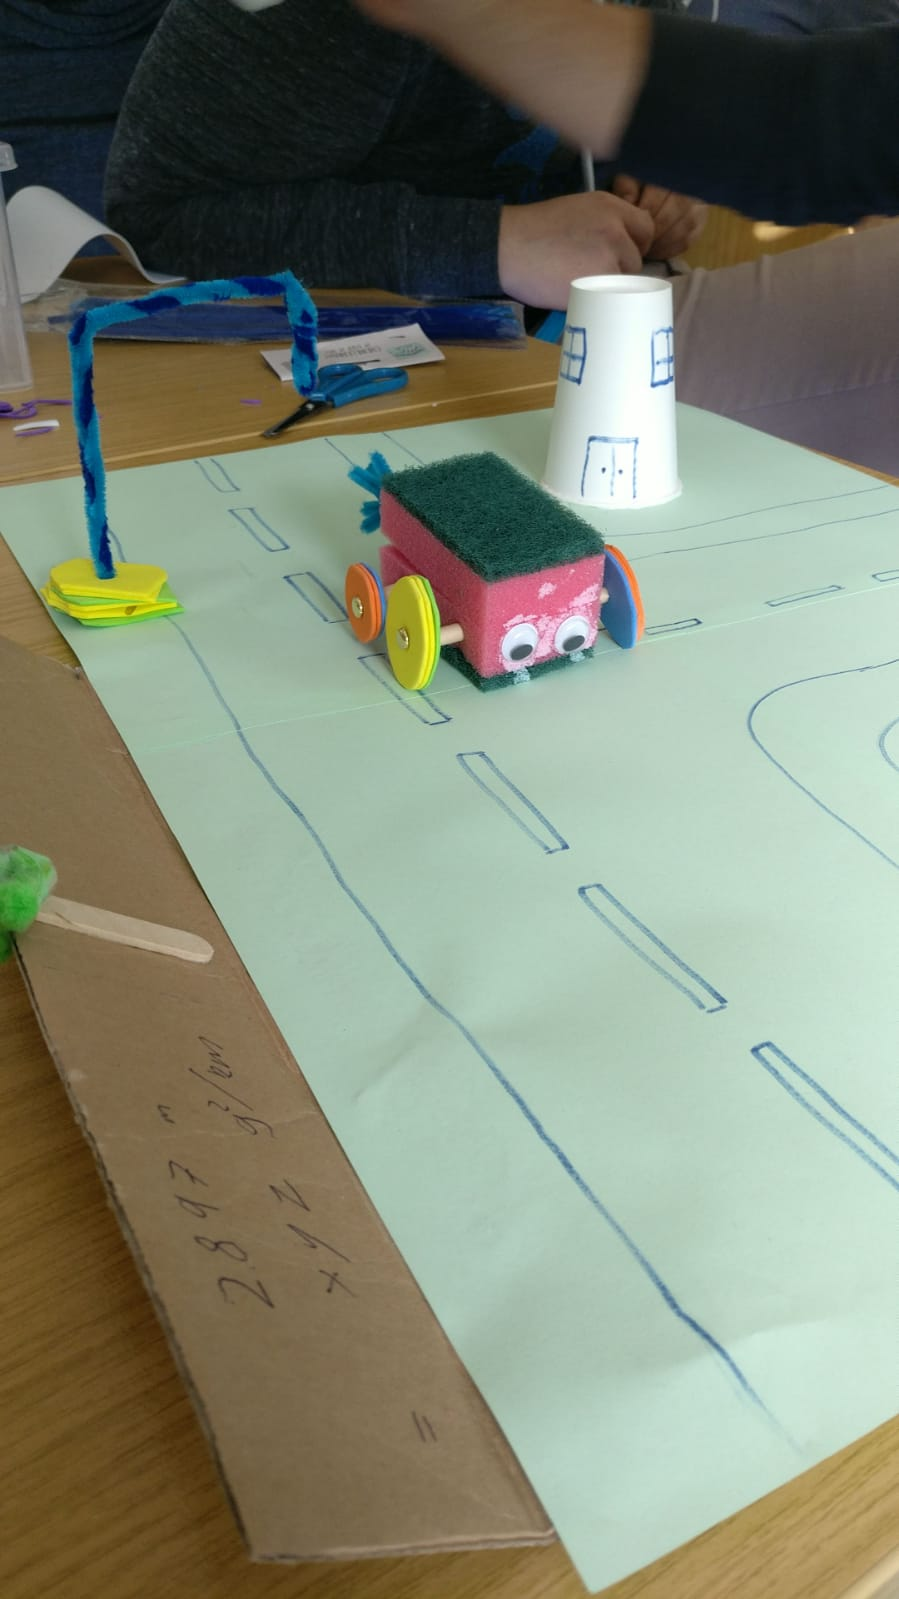
\includegraphics[
        width=0.5\linewidth,
    ]{imgs/sponge_prototype.jpeg}
    \caption{Erster Prototyp}
    \label{fig-sponge}
\end{center}
\end{figure}
\end{document}